\begin{center}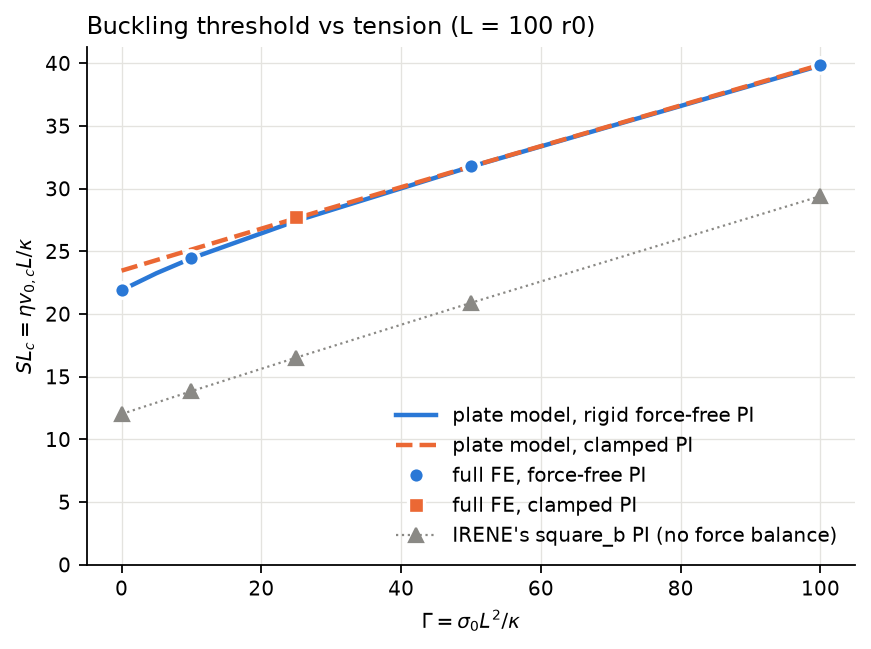
\includegraphics[width=\linewidth,height=175mm,keepaspectratio]{figures/membrane_flow2_threshold_vs_tension.png}\captionof{figure}[Main-text figure, larger copy]{Larger copy of main-text Figure 1. Consult its main-text caption for interpretation. \textit{Source:} \path{research/membrane_stability/figures/flow2_threshold_vs_tension.png}. First added 2026-09-30.}\end{center}\clearpage
\begin{center}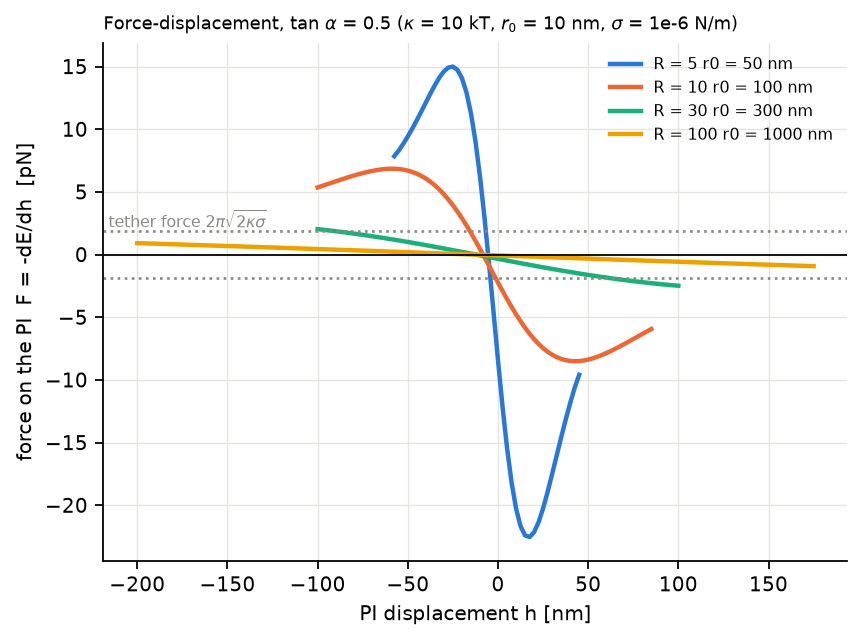
\includegraphics[width=\linewidth,height=175mm,keepaspectratio]{figures/membrane_ring_force_physical_units.png}\captionof{figure}[Main-text figure, larger copy]{Larger copy of main-text Figure 2. Consult its main-text caption for interpretation. \textit{Source:} \path{research/membrane_stability/figures/ring_force_physical_units.png}. First added 2026-09-30.}\end{center}\clearpage
\begin{center}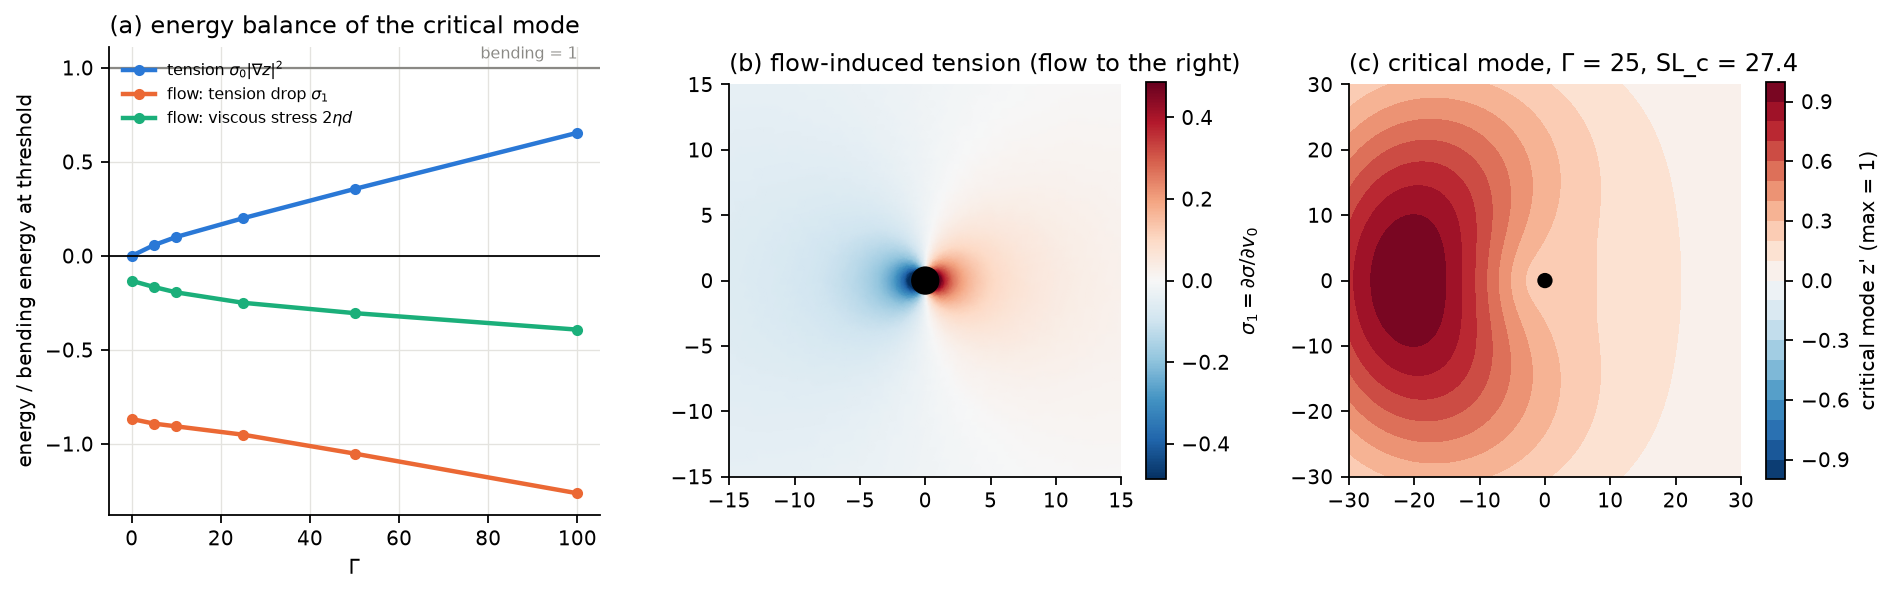
\includegraphics[width=\linewidth,height=175mm,keepaspectratio]{figures/membrane_flow2_plate_model.png}\captionof{figure}[Main-text figure, larger copy]{Larger copy of main-text Figure 3. Consult its main-text caption for interpretation. \textit{Source:} \path{research/membrane_stability/figures/flow2_plate_model.png}. First added 2026-09-30.}\end{center}\clearpage
\begin{center}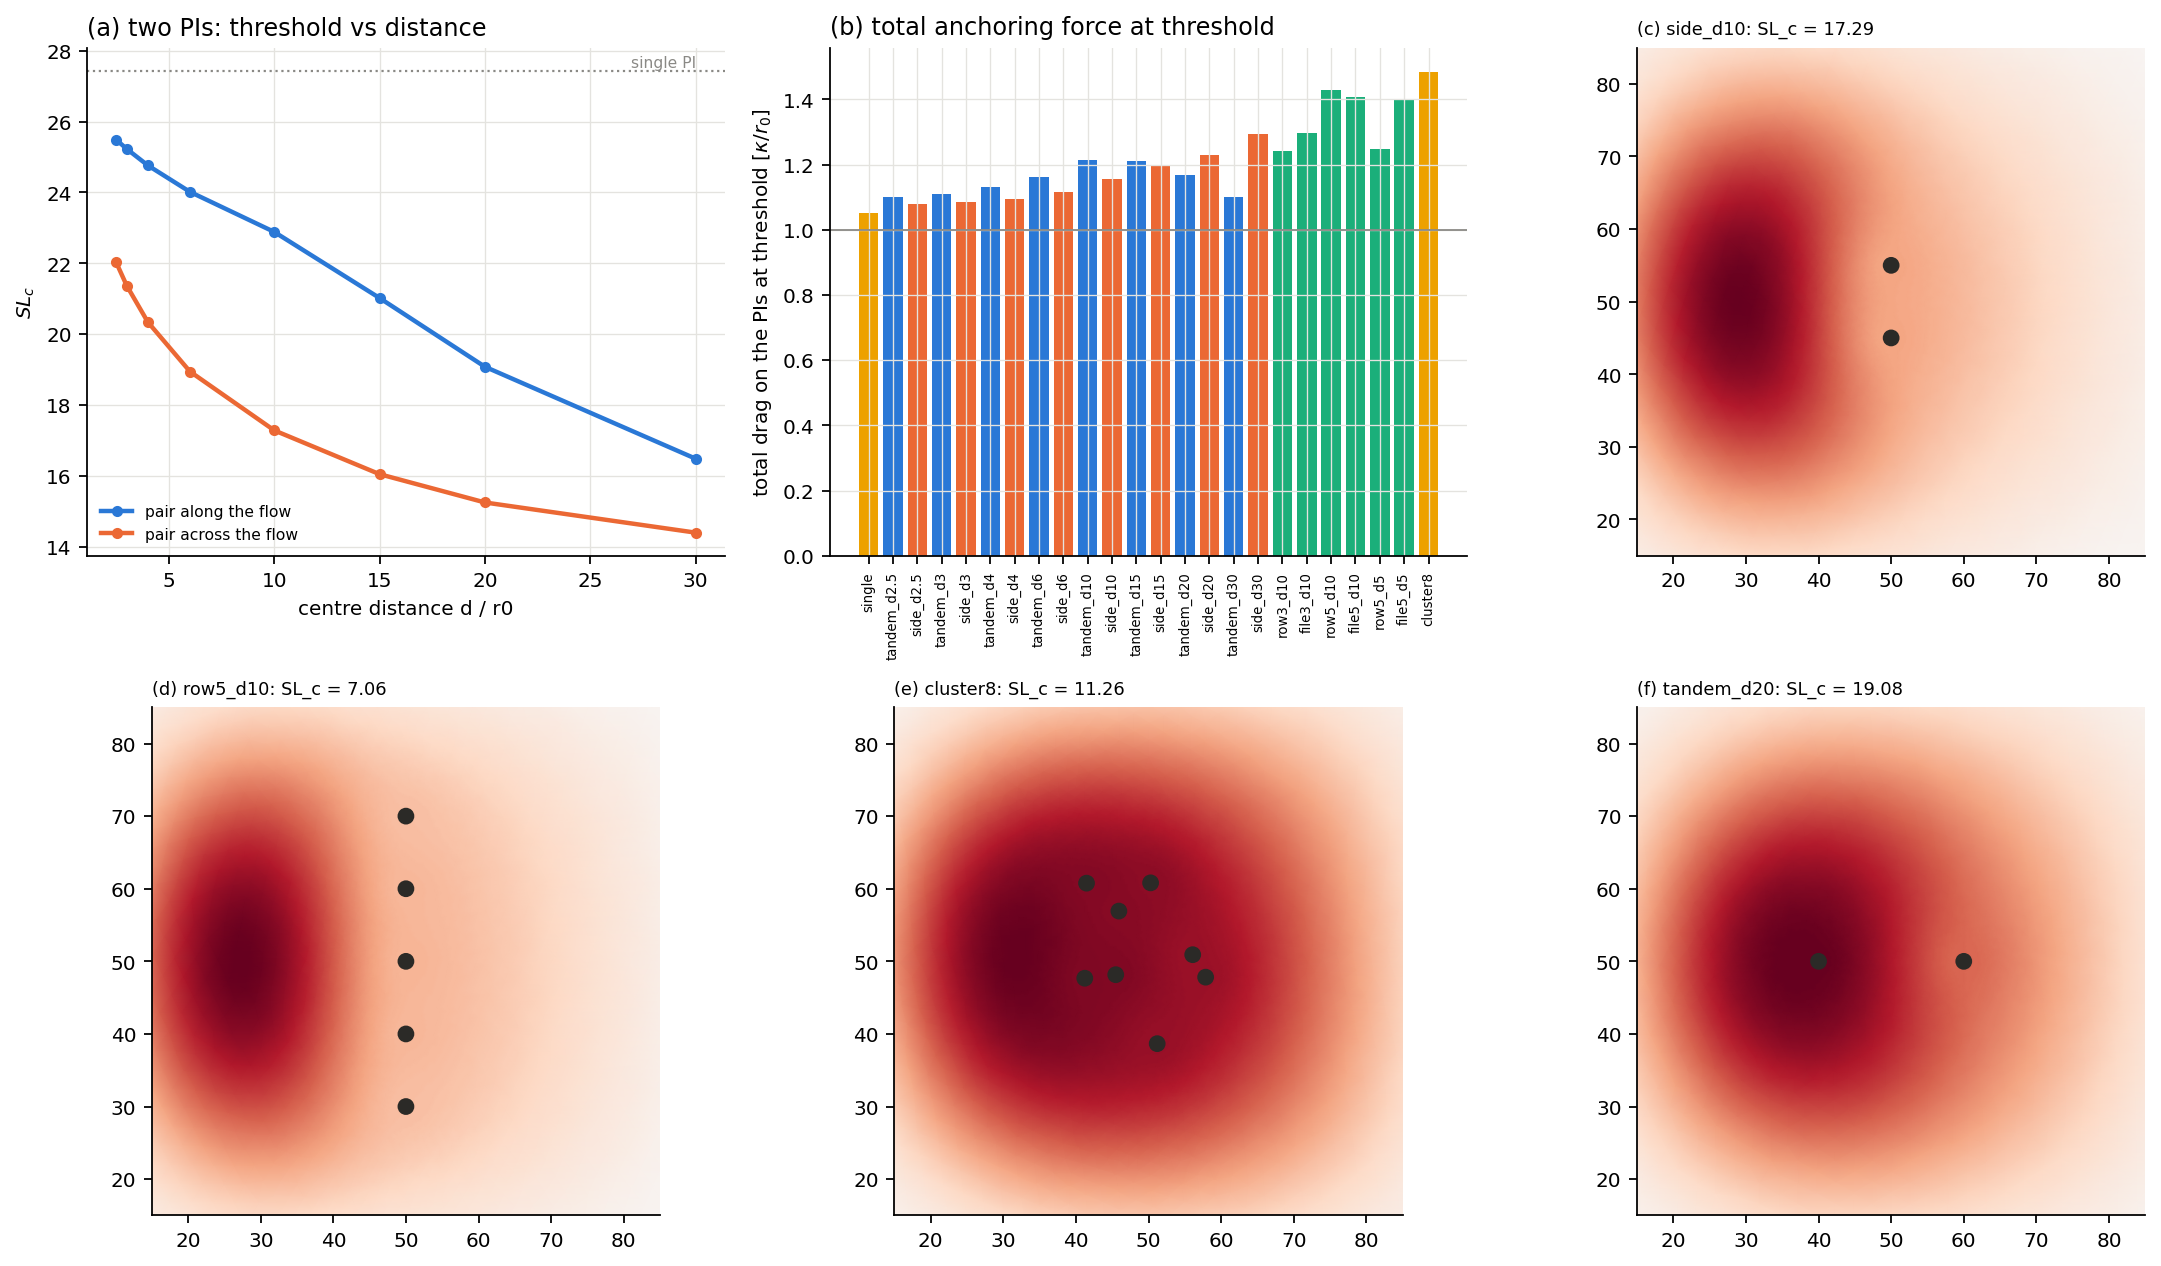
\includegraphics[width=\linewidth,height=175mm,keepaspectratio]{figures/membrane_r3_multi.png}\captionof{figure}[Main-text figure, larger copy]{Larger copy of main-text Figure 4. Consult its main-text caption for interpretation. \textit{Source:} \path{research/membrane_stability/figures/r3_multi.png}. First added 2026-10-01.}\end{center}\clearpage
\begin{center}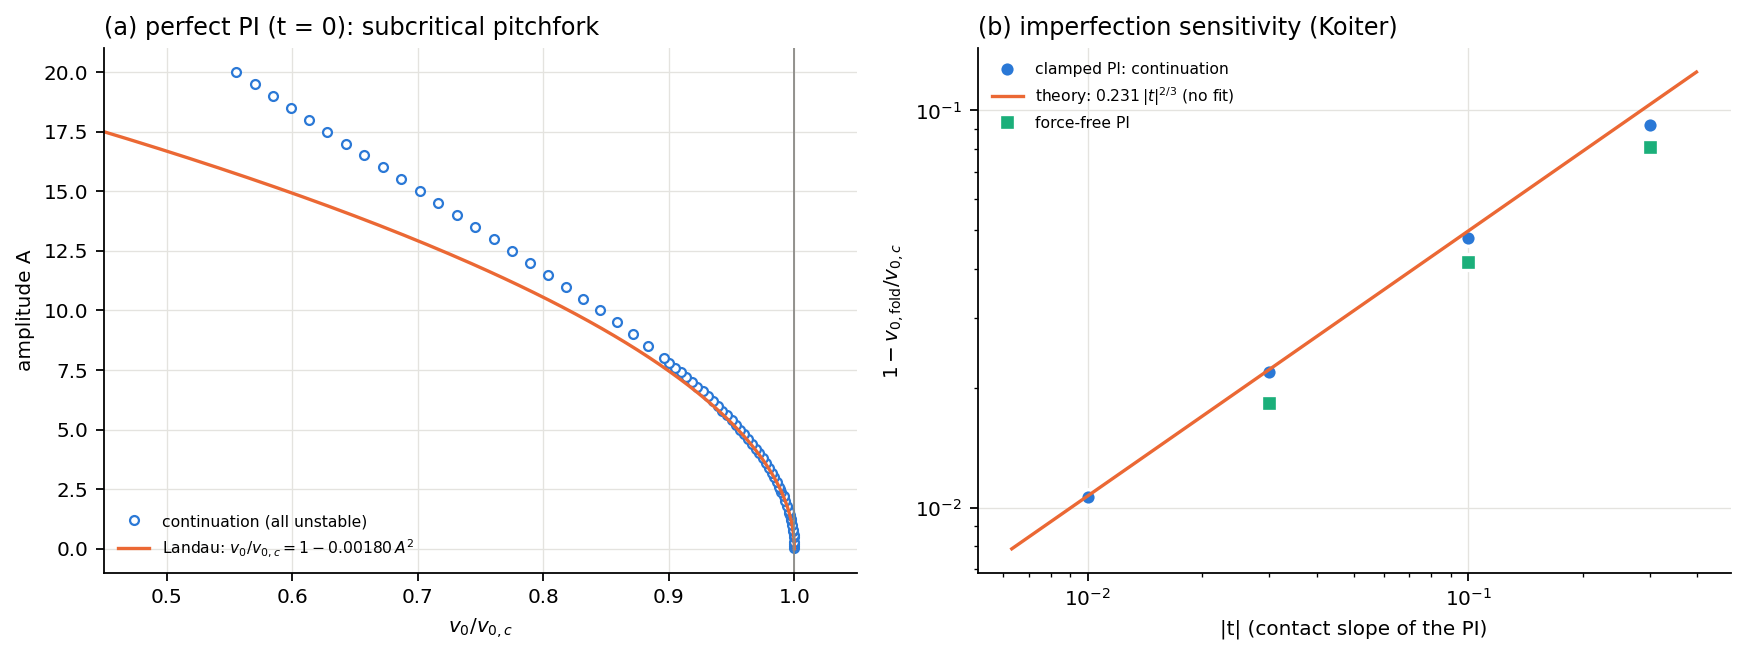
\includegraphics[width=\linewidth,height=175mm,keepaspectratio]{figures/membrane_r3_landau.png}\captionof{figure}[Main-text figure, larger copy]{Larger copy of main-text Figure 5. Consult its main-text caption for interpretation. \textit{Source:} \path{research/membrane_stability/figures/r3_landau.png}. First added 2026-10-01.}\end{center}\clearpage
\begin{center}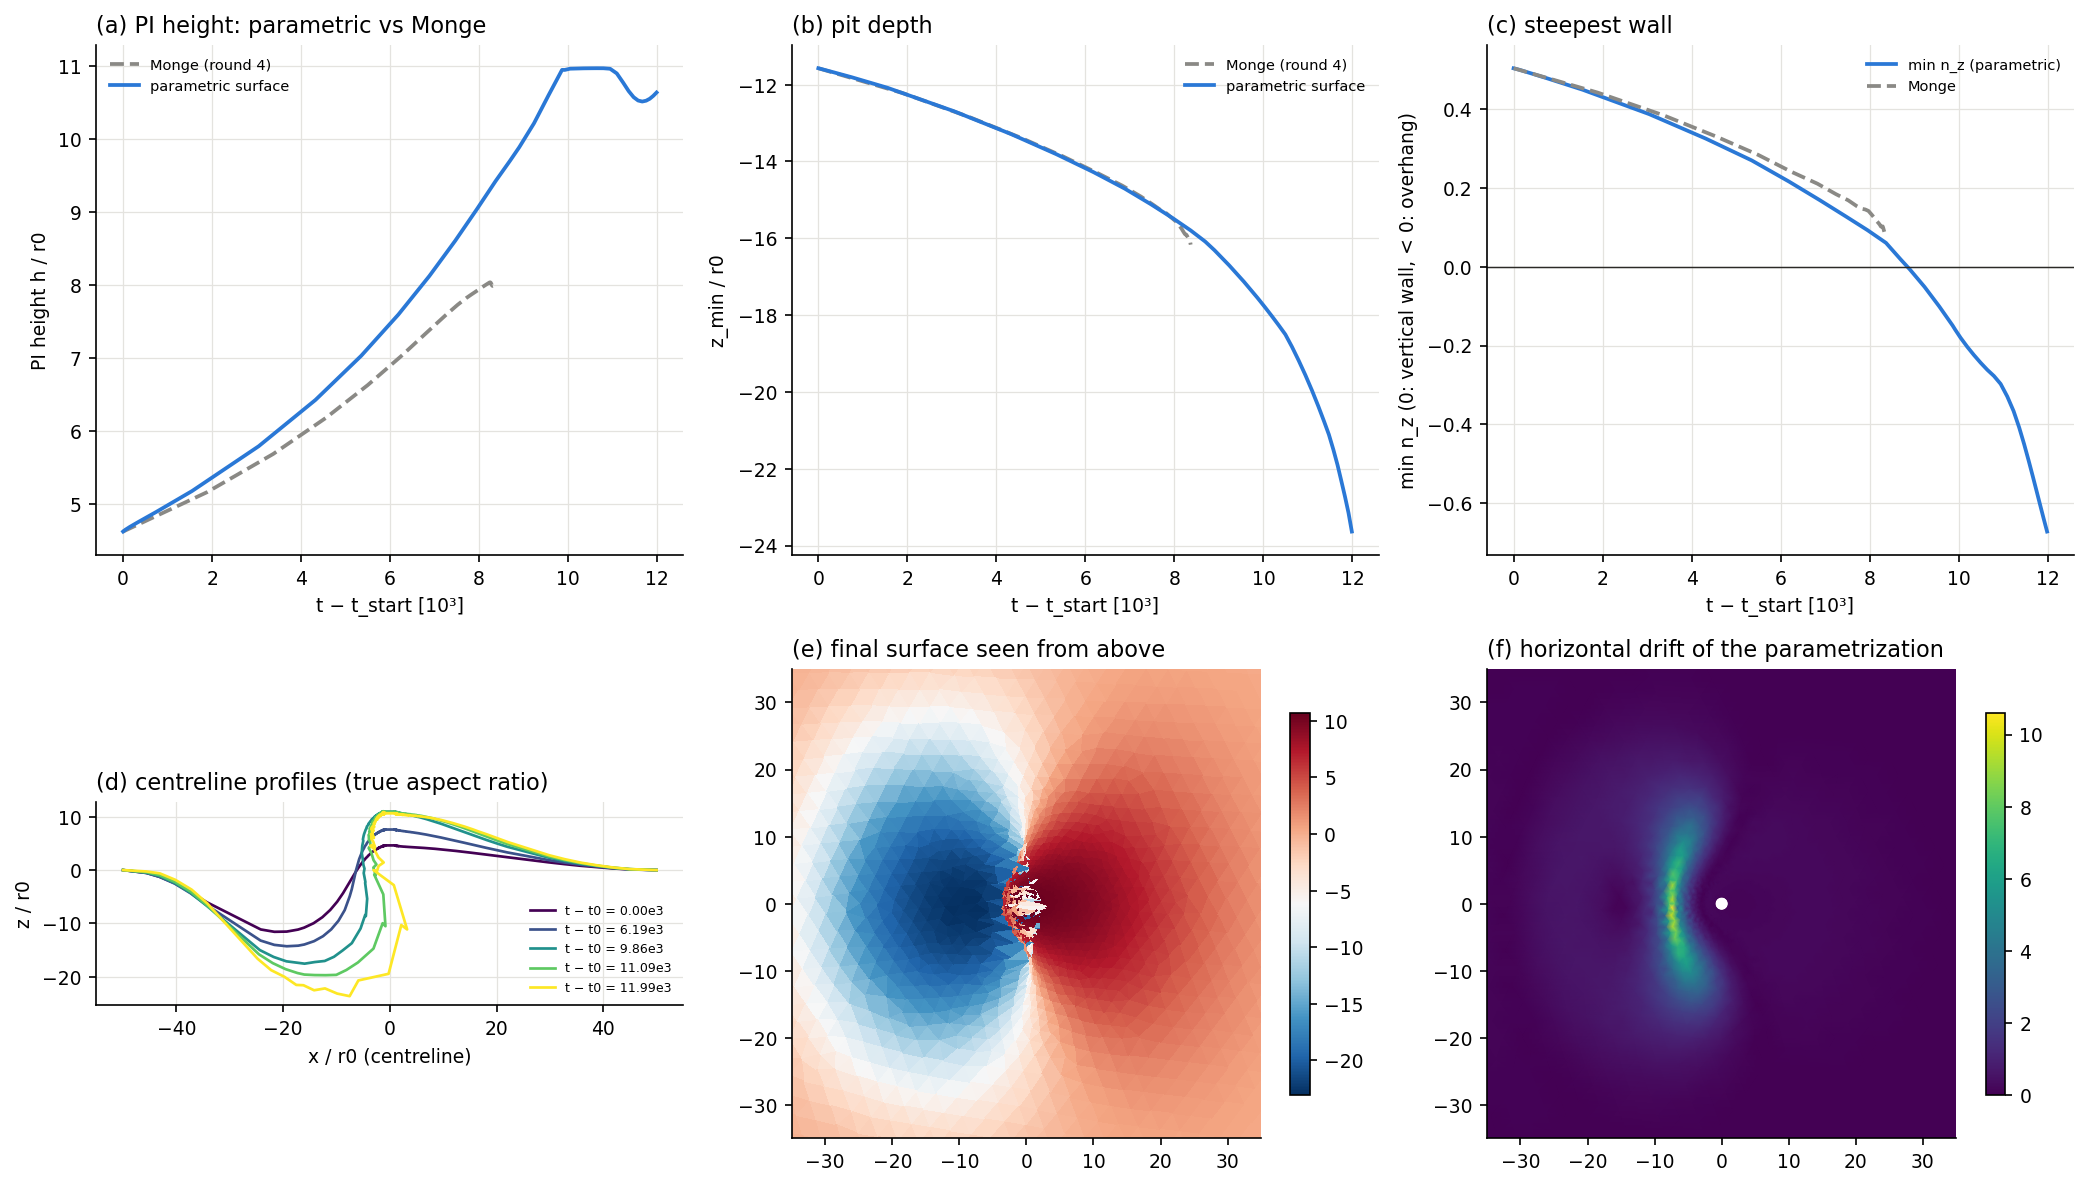
\includegraphics[width=\linewidth,height=175mm,keepaspectratio]{figures/membrane_r5_fold_parametric.png}\captionof{figure}[Main-text figure, larger copy]{Larger copy of main-text Figure 6. Consult its main-text caption for interpretation. \textit{Source:} \path{research/membrane_stability/figures/r5_fold_parametric.png}. First added 2026-10-02.}\end{center}\clearpage
\begin{center}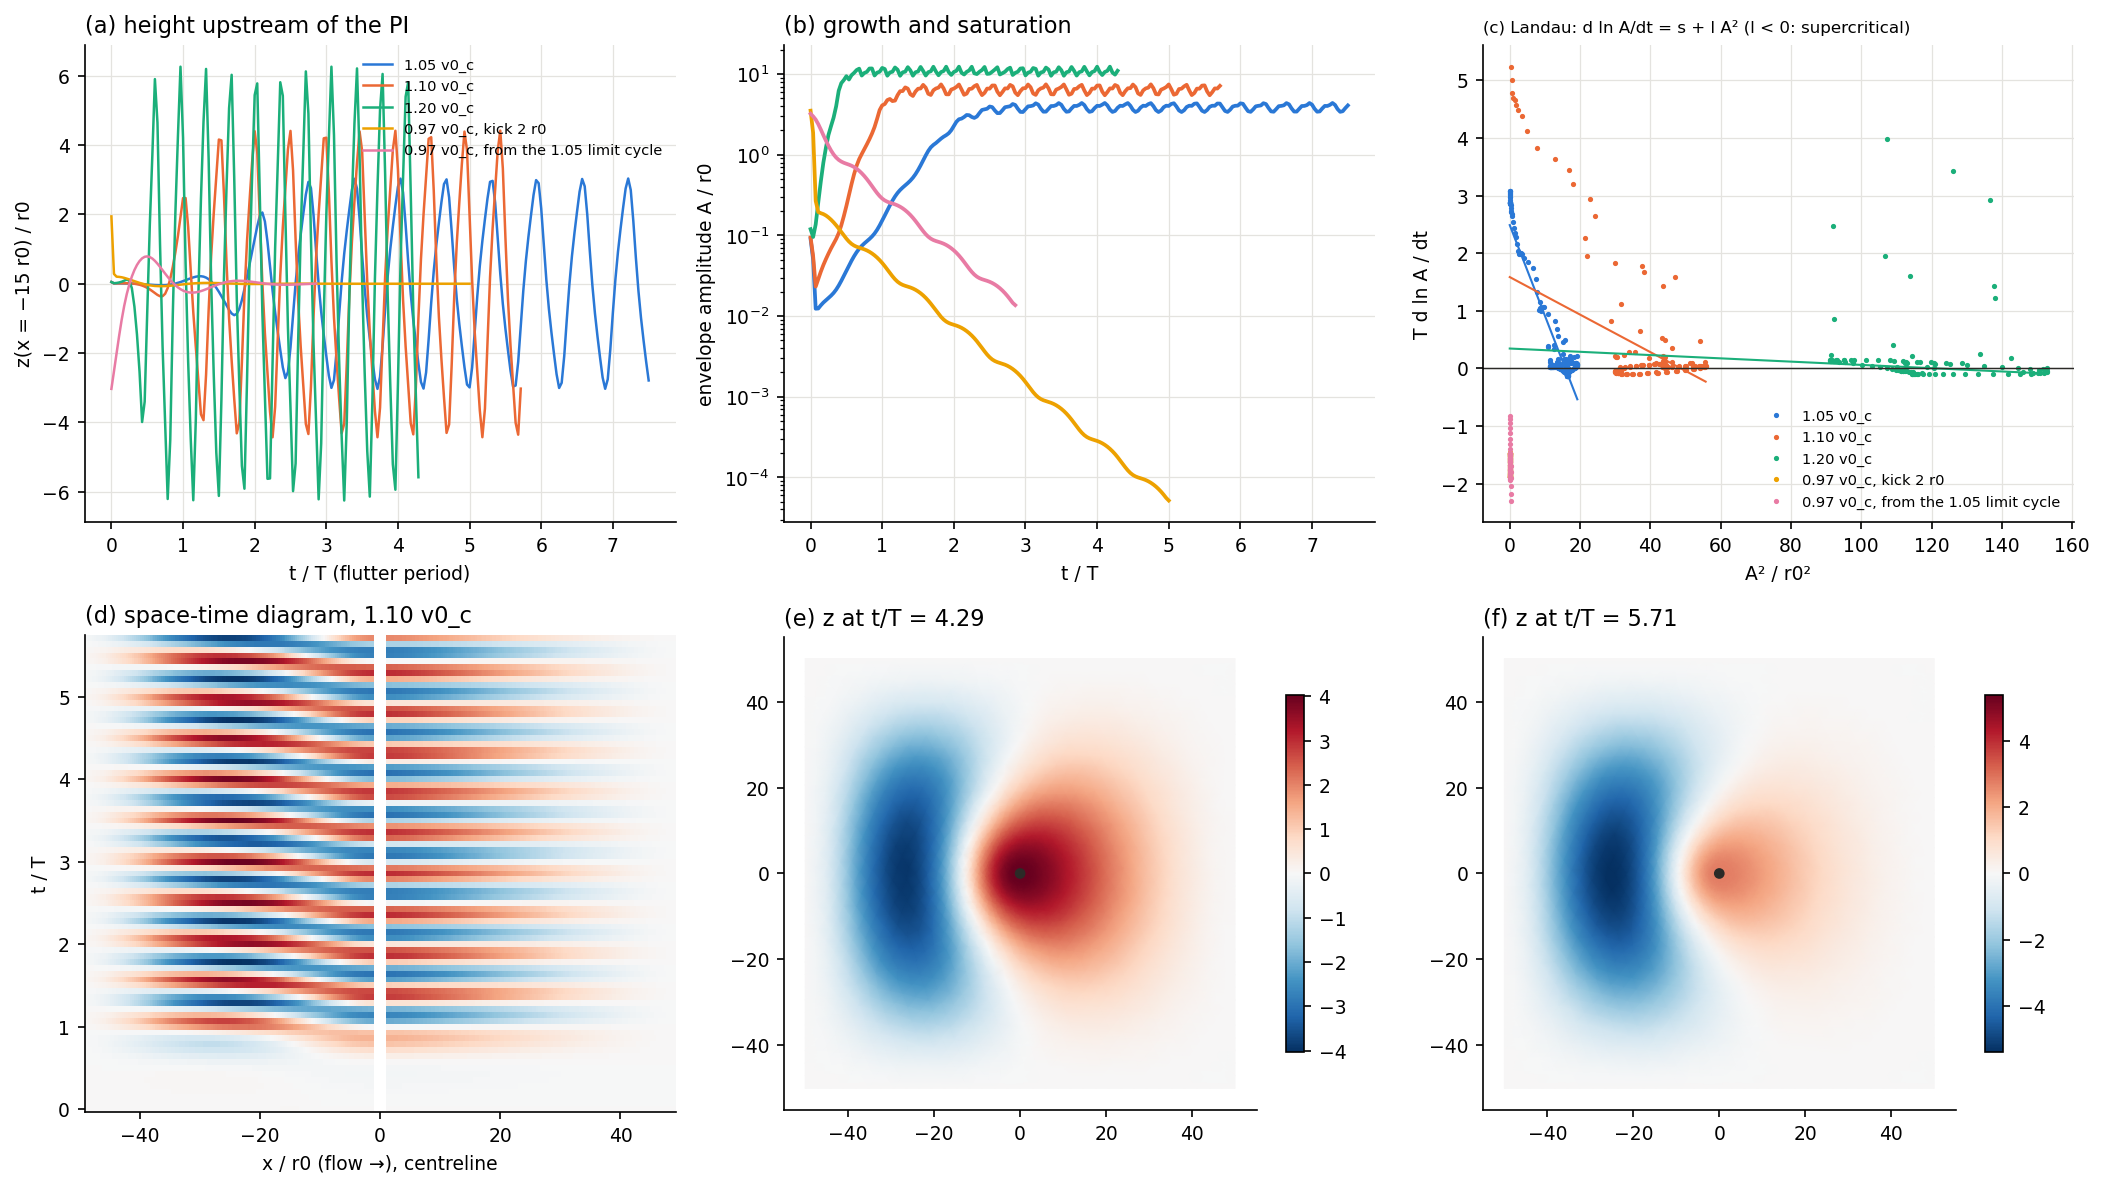
\includegraphics[width=\linewidth,height=175mm,keepaspectratio]{figures/membrane_r5_flutter.png}\captionof{figure}[Main-text figure, larger copy]{Larger copy of main-text Figure 7. Consult its main-text caption for interpretation. \textit{Source:} \path{research/membrane_stability/figures/r5_flutter.png}. First added 2026-10-02.}\end{center}\clearpage
\begin{center}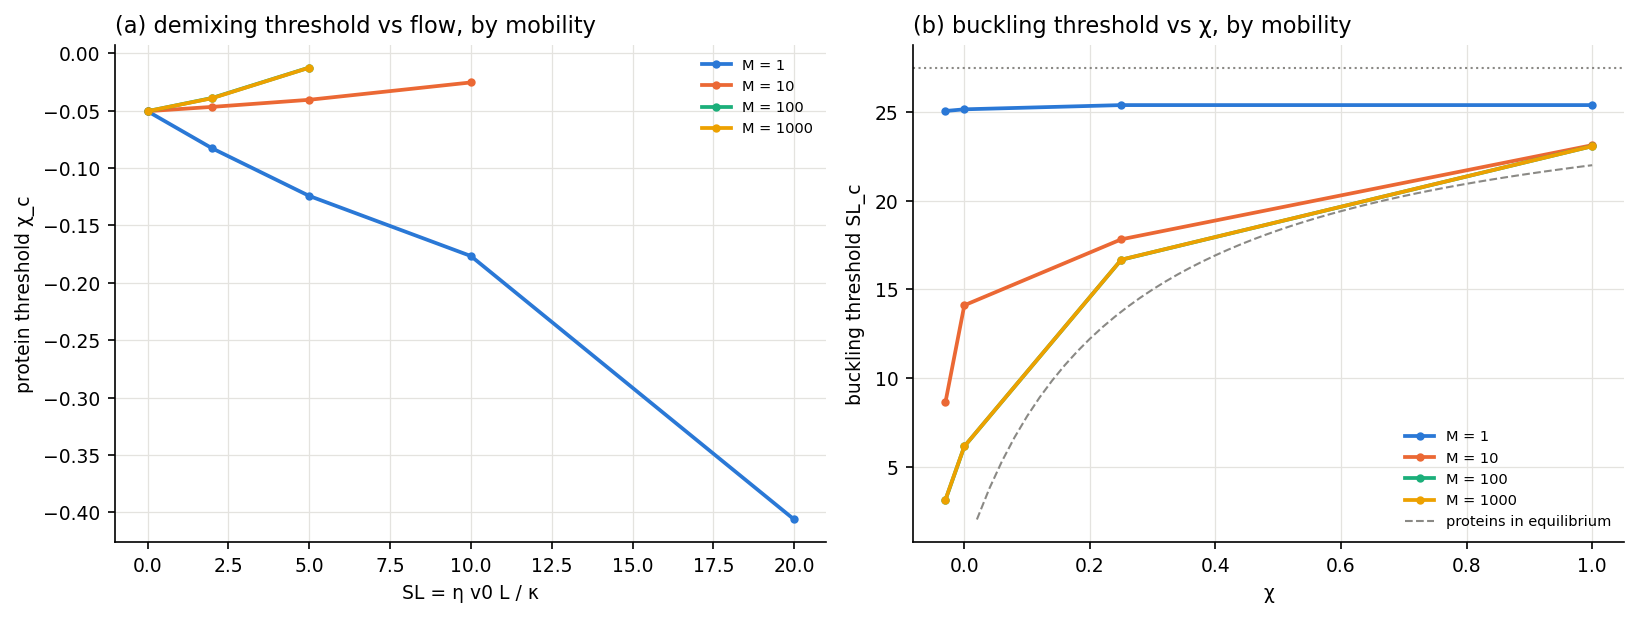
\includegraphics[width=\linewidth,height=175mm,keepaspectratio]{figures/membrane_r5_peclet.png}\captionof{figure}[Main-text figure, larger copy]{Larger copy of main-text Figure 8. Consult its main-text caption for interpretation. \textit{Source:} \path{research/membrane_stability/figures/r5_peclet.png}. First added 2026-10-02.}\end{center}\clearpage
\begin{center}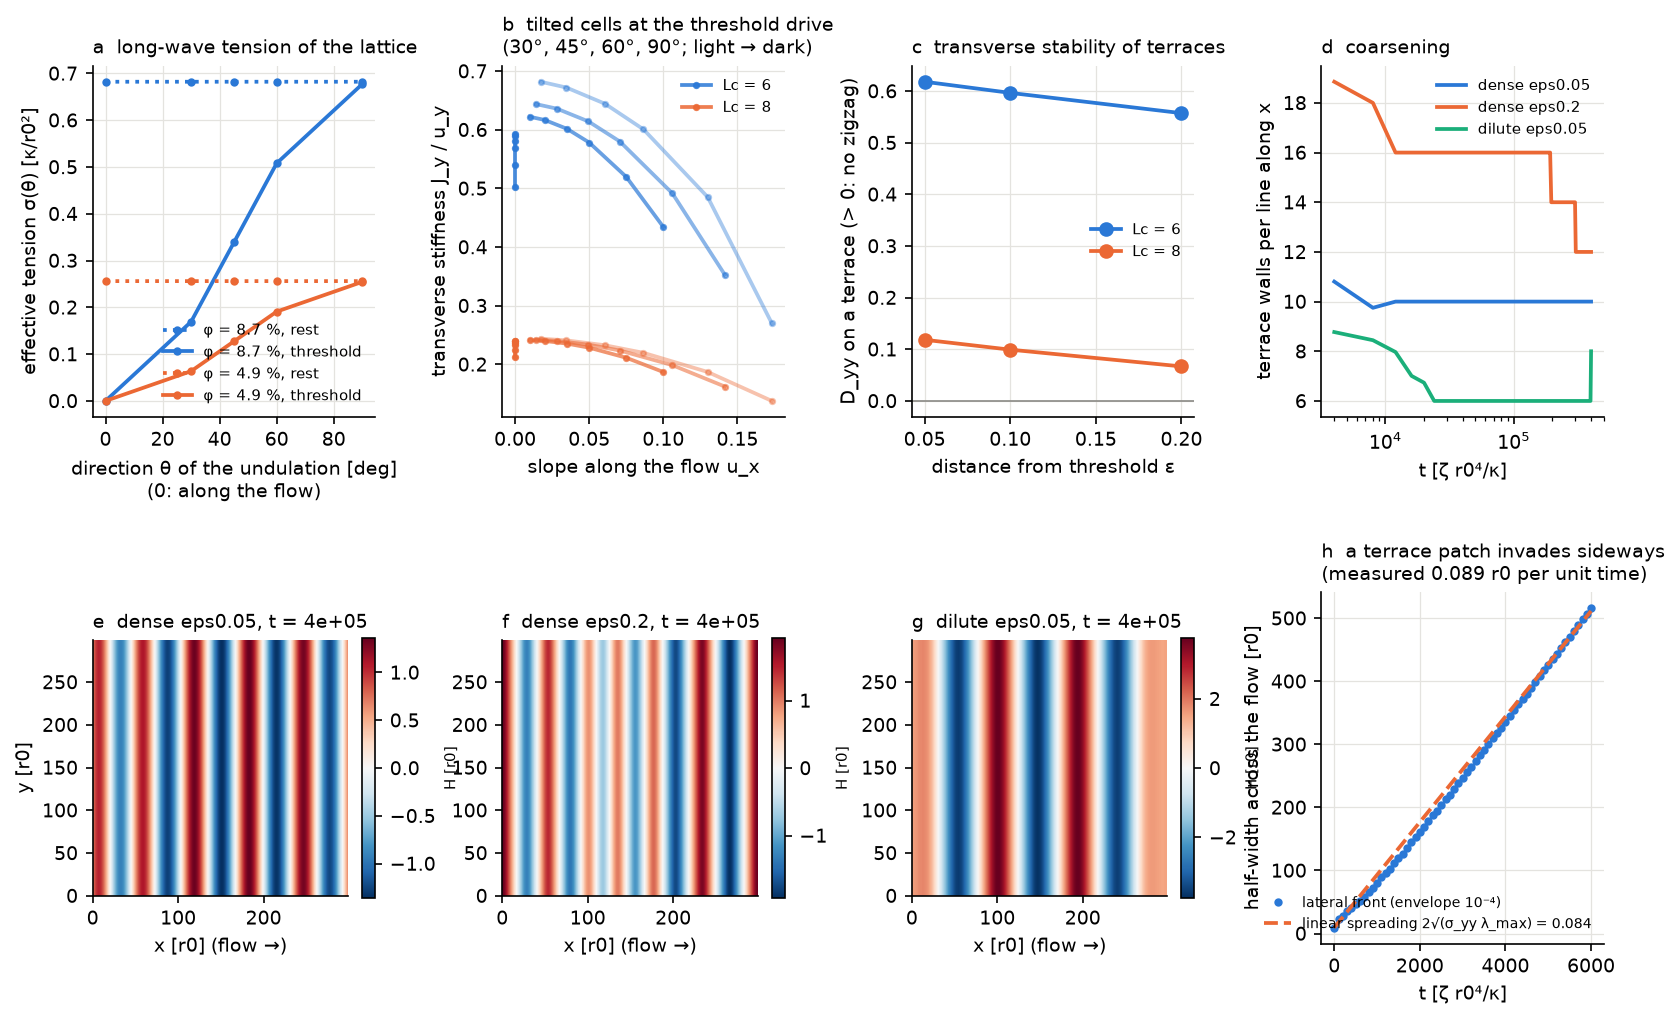
\includegraphics[width=\linewidth,height=175mm,keepaspectratio]{figures/membrane_r6_slope2d.png}\captionof{figure}[Main-text figure, larger copy]{Larger copy of main-text Figure 9. Consult its main-text caption for interpretation. \textit{Source:} \path{research/membrane_stability/figures/r6_slope2d.png}. First added 2026-10-03.}\end{center}\clearpage
